\appendix
\section{Notation}
\label{app:notation}
\begin{table}[h]\centering\small\sffamily
\caption{Symbols used throughout.}
\begin{tabular}{L{2.6cm} L{11.6cm}}
\toprule
\hdr{symbol} & \hdr{meaning}\\
\midrule
\rowcolor{facebg} $i,j,k$ & patient, indicator, specific-dimension indices\\
$N,J,K,F$ & patients ($9{,}013$), indicators, specific dimensions, total factors $F=K{+}1$\\
\rowcolor{facebg} $G_i,\;D_{ik}$ & general-factor and specific-factor scores for patient $i$\\
$\Lambda,\;\lambda_{jG},\;\lambda_{jk}$ & loading matrix; general loading; specific loading of indicator $j$\\
\rowcolor{facebg} $\Phi$ & inter-factor correlation matrix (specific block; $G$ orthogonal in the bifactor)\\
$\Psi=\diagop(\sigma_j^2)$ & diagonal residual-variance matrix; $\sigma_j$ residual scale\\
\rowcolor{facebg} $\alpha_j,\;\beta_j,\;c_i$ & item intercept; covariate coefficients; covariate vector\\
$\eta_{ij}$ & linear predictor for indicator $j$ in patient $i$ (Eq.~\ref{eq:eta})\\
\rowcolor{facebg} $\Obs_i$ & set of indicators observed for patient $i$\\
$\Sigma=\Lambda\Phi\Lambda\Tn+\Psi$ & marginal indicator covariance (continuous block)\\
\rowcolor{facebg} $A_i,\;b_i,\;W_i$ & Woodbury factor-space precision, information vector, observed-cell precision\\
$\widehat{R},\;\mathrm{ESS}$ & potential scale reduction factor; effective sample size\\
\bottomrule
\end{tabular}
\end{table}

\section{The prior atlas}
\label{app:prioratlas}
Figure~\ref{fig:prioratlas} is the theory half of the map (Section~\ref{sec:model}): the soft-prior loading
matrix as an indicator$\times$factor heatmap, generated from configuration alone. Cell shade is the
prior-permitted loading $|\text{mean}|+\text{sd}$: dark $=$ \code{primary}/\code{g_anchor} (theory expects a
loading), mid $=$ \code{plausible_cross} (theory allows), light $=$ soft-zero (suppressed unless the data
surprise the prior). Table~\ref{tab:pool} gives the per-factor prior pool.

\begin{table}[h]\centering\small\sffamily
\caption{Per-factor prior pool: primary indicators and likelihood mix. $143$ indicators $\times\,10$ candidate
factors. Negative symptoms, sensory abnormalities, and impulsivity are absent --- no usable common indicators.}
\label{tab:pool}
\begin{tabular}{L{4.0cm} R{2.0cm} L{8.0cm}}
\toprule
\hdr{factor} & \hdr{primaries} & \hdr{likelihood mix}\\
\midrule
\rowcolor{facebg} $G$ --- severity/burden & 14 & gaussian 11, bernoulli 3 (functioning + severity only)\\
cognition & 11 & gaussian 11 (CVLT/WAIS/fluency/TMT)\\
\rowcolor{facebg} metabolic & 32 & gaussian 19, lognormal 10, bernoulli 3\\
inflammatory & 14 & lognormal 8, bernoulli 6\\
\rowcolor{facebg} sleep & 9 & gaussian 9 (PSQI + ESS/CSM)\\
suicidality & 30 & bernoulli 14, ordered-logistic 14, gaussian 1, neg-binomial 1\\
\rowcolor{facebg} developmental-risk & 23 & gaussian 12, bernoulli 8, ordered-logistic 3\\
anhedonia & 1 & gaussian 1 (thin)\\
\rowcolor{facebg} mania-activation & 2 & gaussian 2 (candidate)\\
substance & 4 & bernoulli 2, gaussian 1, neg-binomial 1 (candidate)\\
\rowcolor{facebg} cross-loading windows & --- & MADRS/QIDS/STAI $\to$ plausible on $G$, sleep, cognition, $\dots$\\
\bottomrule
\end{tabular}
\end{table}

\begin{figure}[p]\centering
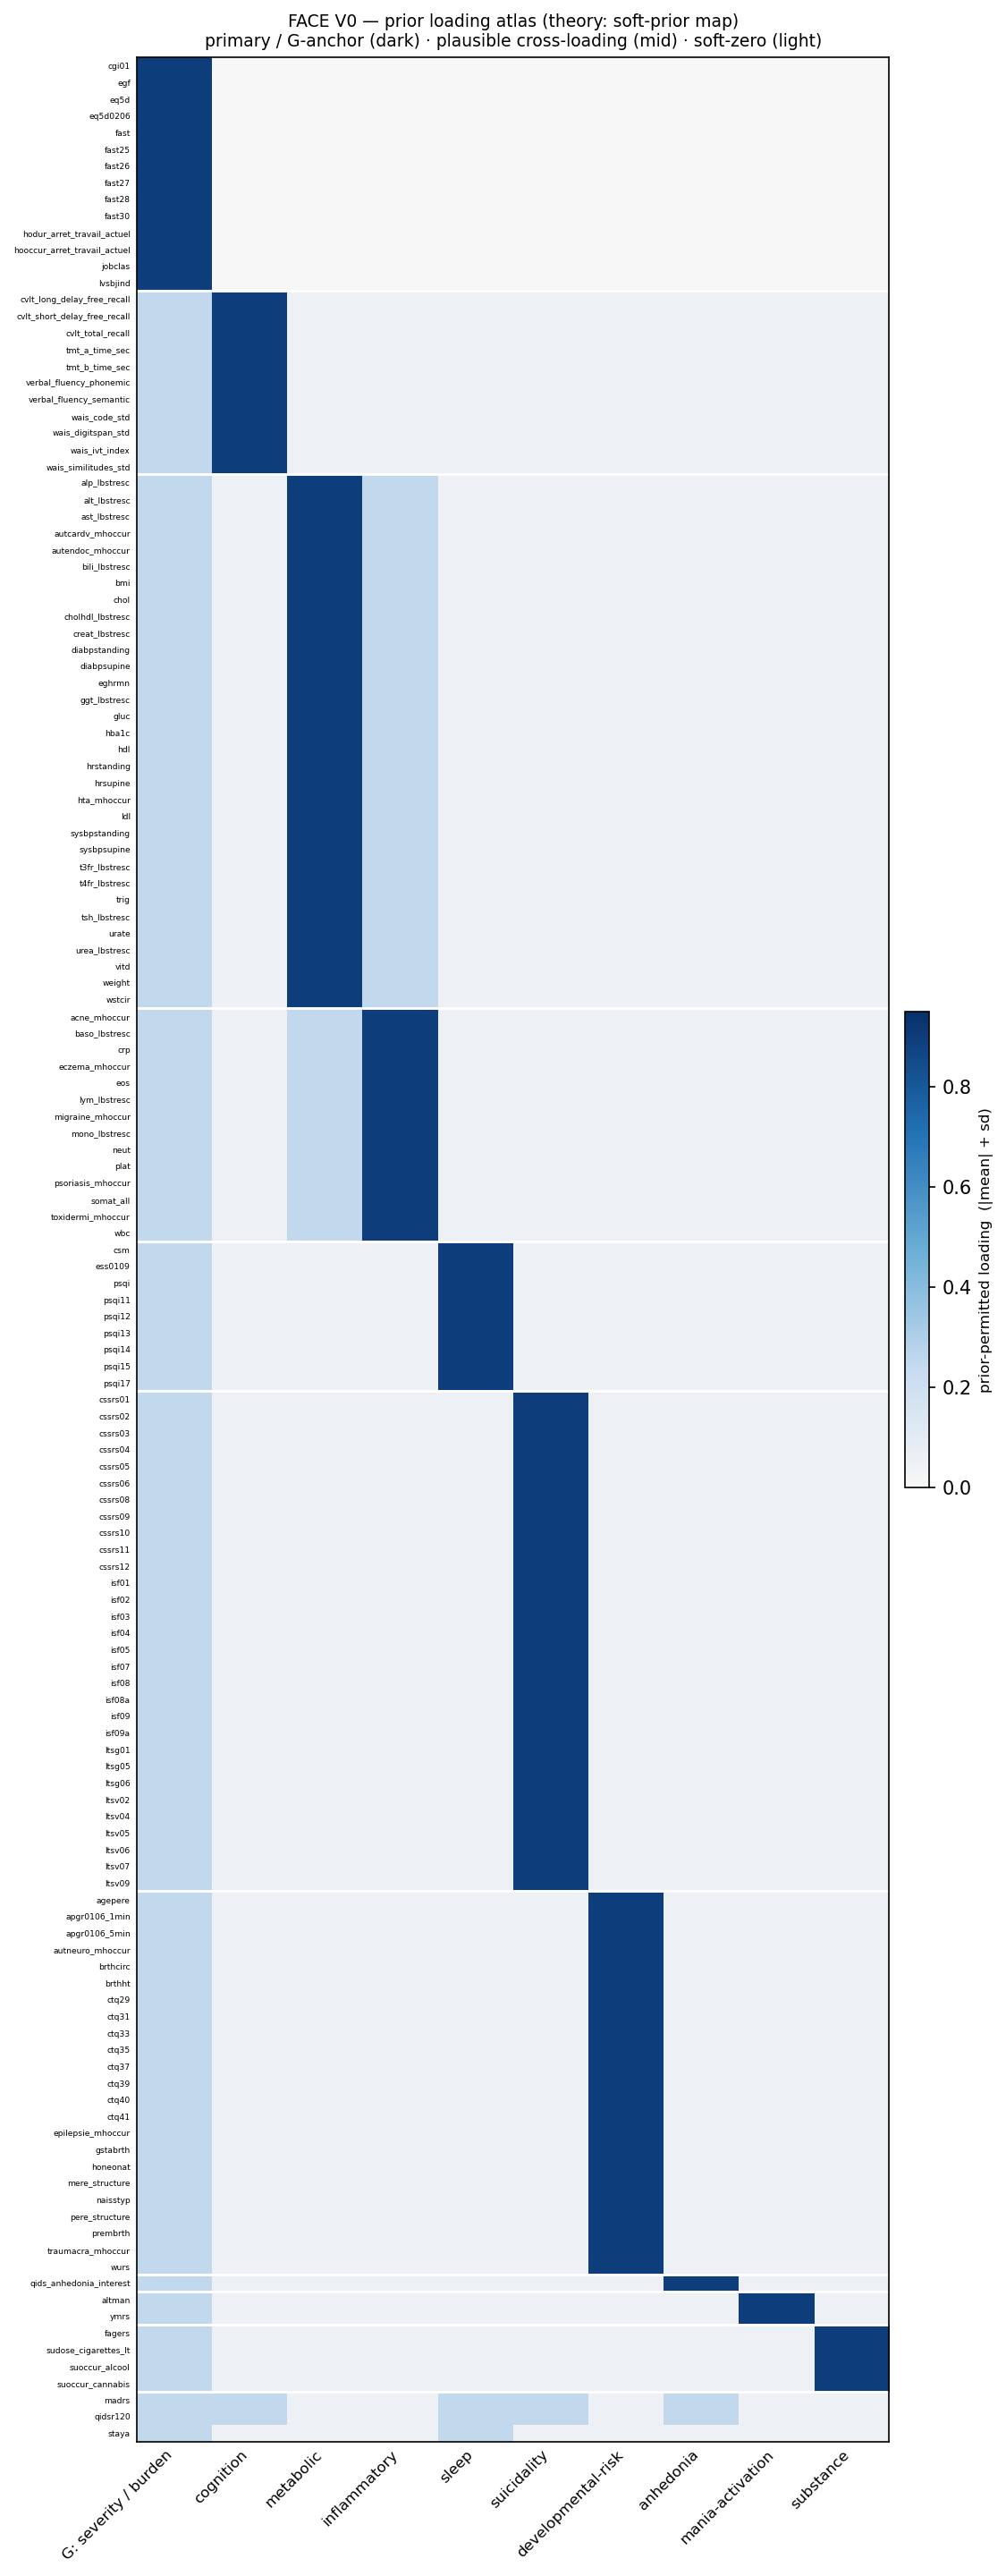
\includegraphics[height=0.84\textheight,keepaspectratio]{figures/prior_atlas.png}
\caption{The prior loading atlas (theory). Rows: the $143$ modelled indicators, grouped by home factor.
Columns: the $10$ candidate factors. The block-diagonal primaries, the faint $G$ column over every specific
item (the bifactor mechanism), and the homeless cross-loading windows (bottom) are all visible. The empirical
atlas --- the fitted posterior loadings beside this map, with per-candidate verdicts --- is the M1 deliverable
(Section~\ref{sec:roadmap}).}
\label{fig:prioratlas}
\end{figure}

\section{Acceptance gates and sampler diagnostics}
\label{app:gates}
A stage is \certified\ only if it passes all gates; otherwise it is \provisional.
\begin{table}[h]\centering\small\sffamily
\caption{The acceptance gate and the diagnostics it reads.}
\begin{tabular}{L{3.4cm} L{4.0cm} L{6.6cm}}
\toprule
\hdr{diagnostic} & \hdr{gate} & \hdr{what it detects}\\
\midrule
\rowcolor{facebg} $\widehat{R}$ (R-hat) & $\le 1.01$ & between- vs.\ within-chain disagreement (non-mixing)\\
ESS (bulk \& tail) & $\ge 400$ & effective independent draws after autocorrelation\\
\rowcolor{facebg} divergences & $=0$ & Hamiltonian integration failing on pathological geometry\\
Heywood & $\max_j|\lambda_j|$ capped & loadings explaining too much / residual collapse\\
\rowcolor{facebg} PPC (Bayesian SRMR) & not grossly violated & absolute fit: model-implied vs.\ observed correlations\\
WAIC & lower preferred & out-of-sample predictive fit for model comparison\\
\rowcolor{facebg} Tucker $\varphi$ & $\ge 0.95$ invariant & loading-pattern congruence (robustness / invariance)\\
\bottomrule
\end{tabular}
\end{table}

\section{Glossary of instruments and abbreviations}
\label{app:glossary}
{\small
\textbf{Cohorts \& design.} BP bipolar disorder; SZ schizophrenia; DR depression; V0 baseline visit; FACE the
harmonized three-cohort expert-centre database.\\[3pt]
\textbf{Frameworks.} RDoC Research Domain Criteria; HiTOP Hierarchical Taxonomy of Psychopathology; ESEM
exploratory structural equation modelling; FIML full-information maximum likelihood.\\[3pt]
\textbf{Functioning \& severity ($G$).} FAST Functioning Assessment Short Test; EGF (\'evaluation globale du
fonctionnement / GAF); EQ-5D EuroQol; CGI-S Clinical Global Impression -- Severity.\\[3pt]
\textbf{Cognition.} WAIS Wechsler Adult Intelligence Scale; TMT Trail Making Test; CVLT California Verbal
Learning Test.\\[3pt]
\textbf{Specific domains.} PSQI Pittsburgh Sleep Quality Index; CTQ Childhood Trauma Questionnaire; WURS
Wender Utah Rating Scale; ISF self-report suicidality items; C-SSRS Columbia Suicide Severity Rating Scale.\\[3pt]
\textbf{Windows.} MADRS Montgomery--\AA sberg Depression Rating Scale; QIDS Quick Inventory of Depressive
Symptomatology; STAI State--Trait Anxiety Inventory.\\[3pt]
\textbf{Statistics.} NUTS No-U-Turn Sampler; LKJ Lewandowski--Kurowicka--Joe correlation prior; WAIC widely
applicable information criterion; SRMR standardized root-mean-square residual; DIF differential item
functioning; ESS effective sample size; $\widehat{R}$ potential scale reduction factor.}
